\documentclass[12pt]{scrartcl}
\usepackage[german, ngerman]{babel}
\usepackage{graphicx}
\usepackage{color}
\usepackage{url}
\usepackage{xcolor}
\usepackage{listings}
\usepackage{hyperref}
\usepackage{nameref}
\usepackage{varioref}

\usepackage[headsepline,footsepline]{scrlayer-scrpage}
\usepackage{biblatex}
\usepackage{amsmath}
\usepackage{float}

\newcommand{\code}[1]{\texttt{#1}}


\definecolor{mGreen}{rgb}{0,0.6,0}
\definecolor{mGray}{rgb}{0.5,0.5,0.5}
\definecolor{mPurple}{rgb}{0.58,0,0.82}
\definecolor{backgroundColour}{rgb}{0.95,0.95,0.95} %{cmyk}{0.05,0.05,0.05,0.05}

\lstdefinestyle{CStyle}{
    backgroundcolor=\color{backgroundColour},
    commentstyle=\color{mGreen},
    keywordstyle=\color{blue},
    numberstyle=\tiny\color{mGray},
    stringstyle=\color{mPurple},
    basicstyle=\footnotesize,
    breakatwhitespace=false,
    breaklines=true,
    captionpos=b,
    keepspaces=true,
    numbers=left,
    numbersep=5pt,
    showspaces=false,
    showstringspaces=false,
    showtabs=false,
    tabsize=2,
    language=C++
}

\lstdefinestyle{Terminal}{
    backgroundcolor=\color{backgroundColour},
    commentstyle=\color{black},
    keywordstyle=\color{black},
    numberstyle=\tiny\color{black},
    stringstyle=\color{black},
    basicstyle=\footnotesize,
    breakatwhitespace=false,
    breaklines=true,
    captionpos=b,
    keepspaces=true,
    numbers=none,
    numbersep=5pt,
    showspaces=false,
    showstringspaces=false,
    showtabs=false,
    tabsize=2,
}


\pagestyle{scrheadings}
\clearscrheadfoot
%\cfoot{Tobias Gruber}
\cfoot{\pagemark}
\chead{\headmark}
\automark[subsection]{section}


\begin{document}


\begin{titlepage}
    \vfill
	\centering
    \vspace{1.5cm}

	{\scshape\LARGE Hochschule München \par}
    {\scshape\Large Fakultät für Informatik und Mathematik\par}
	\vspace{1.5cm}




    \vfill
    {\LARGE\bfseries Praktikumsaufgabe 2 \\}
    \vspace{0.5cm}
	{in der Vorlesung\\}
    \vspace{0.5cm}
    {\LARGE\bfseries Computational Geometry\\~\\ \par}
	{\LARGE Fläche, Volumen, Modellierung\\~\\ \par}
	\vfill
    \vfill


    \begin{tabular}{ll}
    \normalsize
    Team:  & Christopher Hinz, Tobias Gruber\\
    Studiengruppe: & Master Informatik\\
    Studiensemester: & 1. Semester\\
    Schwerpunkt: & Embedded Computing\\
    \end{tabular}
    \vspace{1.5cm}

    \today

    \vspace{0.5cm}

    Sommersemester 2022

	\vfill

\end{titlepage}

\newpage



\raggedright

%%%%%%%%%%%%%%%%%%%%%%%%%%%%%
% Problemstellung
%%%%%%%%%%%%%%%%%%%%%%%%%%%%%
\section{Problemstellung}
Für dieses Praktikum wurde eine SVG-Datei 'DeutschlandMitStaedten.svg' zur Verfügung gestellt. Ziel der Aufgabe ist es die Flächen der einzelnen Bundesländer (bezüglich der in der Datei verwendeten Skala) zu ermitteln.
Am Ende der Datei befinden sich Koordinaten von Städten. Für diese soll festgestellt werden, in welchem Bundesland die Hauptstadt liegt.


%%%%%%%%%%%%%%%%%%%%%%%%%%%%%
% Umsetzung
%%%%%%%%%%%%%%%%%%%%%%%%%%%%%
\section{Umsetzung}

Für jedes Bundesland gibt es eine Instanz der Klasse bundesland, die in ihrem Konstruktor das nächste Bundesland aus der SVG-Datei ausliest.
Die Bundesländer werden in einem Vektor bundeslaender gespeichert.
Zum Einlesen der svg-Datei wird auf die Parser-Funktionen der RapidXML Library zurückgeriffen.

\ \\~\\

Die Berechnung der Fläche der Bundesländer erfolgt ebenso im Konstruktor der Klasse bundesland.
Da ein Bundesland aus mehreren Polygonen bestehen kann werden diese aufaddiert.
Da es auch vorkommen kann, dass die Vertizes der Polygone in verkehrter Reihenfolge angeordnet sind (gegen den Uhrzeigersinn), wird für die Addition der Polygone der Betrag der Flächen verwendet.

Ebenso können Polygone Löcher enthalten. Diese werden über einen Point-in-Polygon-Test mit einem beliebigen Punkt des zu testenden Polygons bestimmt.
Die Fläche des Polygons wird dann zu der Gesamtfläche nicht aufaddiert, sondern abgezogen.

\ \\~\\

Die Städte werde getrennt von den Bundesländern importiert und in Instanzen der Klasse staedte gespeichert.
Jede Stadt wird mit einem Point-in-Polygon-Test darauf getestet, ob sie in einem der Bundesländer liegt.
Ist dies der Fall, so wird sie der Bundesland-Instanz hinzugefügt.
Hierbei werden die Städte nicht auf die Löcher der Polygone getestet, da dann zum Beispiel Berlin als Hauptstadt von Brandenburg erkannt werden würde.

\section{Ergebnisse}
Nachfolgen ist die Ausgabe des Programmes bundeslaender.cpp dargestellt.

\begin{lstlisting}[style=Terminal, caption={bundeslaender.cpp: Ausgabe Konsole},captionpos=b, label={lst:ausgabe}]
Bundesland: Thueringen
Anzahl der Polygone: 1
Gesamtflaeche: 13724.6
Hauptstadt: Erfurt

Bundesland: Schleswig-Holstein
Anzahl der Polygone: 11
Gesamtflaeche: 13456.4
Hauptstadt: Kiel

Bundesland: Sachsen-Anhalt
Anzahl der Polygone: 1
Gesamtflaeche: 17450.5
Hauptstadt: Magdeburg

Bundesland: Sachsen
Anzahl der Polygone: 1
Gesamtflaeche: 15667.9
Hauptstadt: Dresden

Bundesland: Saarland
Anzahl der Polygone: 1
Gesamtflaeche: 2179.76
Hauptstadt: Saarbruecken

Bundesland: Rheinland-Pfalz
Anzahl der Polygone: 1
Gesamtflaeche: 16913.6
Hauptstadt: Mainz

Bundesland: Nordrhein-Westfalen
Anzahl der Polygone: 1
Gesamtflaeche: 28966.4
Hauptstadt: Duesseldorf

Bundesland: Niedersachsen
Anzahl der Polygone: 10
Gesamtflaeche: 40408.7
Hauptstadt: Hannover

Bundesland: Mecklenburg-Vorpommern
Anzahl der Polygone: 7
Gesamtflaeche: 19658.8
Hauptstadt: Schwerin

Bundesland: Hessen
Anzahl der Polygone: 1
Gesamtflaeche: 17977.5
Hauptstadt: Wiesbaden

Bundesland: Hamburg
Anzahl der Polygone: 1
Gesamtflaeche: 633.325
Hauptstadt: Hamburg

Bundesland: Bremen
Anzahl der Polygone: 2
Gesamtflaeche: 340.931
Hauptstadt: Bremen

Bundesland: Brandenburg
Anzahl der Polygone: 2
Gesamtflaeche: 25275.9
Hauptstadt: Potsdam

Bundesland: Berlin
Anzahl der Polygone: 1
Gesamtflaeche: 766.233
Hauptstadt: Berlin

Bundesland: Bayern
Anzahl der Polygone: 1
Gesamtflaeche: 60026.1
Hauptstadt: Muenchen

Bundesland: Baden Wuerttemberg
Anzahl der Polygone: 2
Gesamtflaeche: 30522.3
Hauptstadt: Stuttgart
\end{lstlisting}

\section{Verifikation und Validierung}
Im vorhergehenden Listing ist zunächst zu erkennen, dass alle Hauptstädte den Bundesländern korrekt zugeordnet wurden (Bei 16 Städen per Sichtkontrolle möglich).
Zur Überprüfung, ob die Flächen der Bundesländer korrekt berechnet wurden, wurde zunächst ein Vorfaktor eingeführt, der es ermöglicht die Flächen der Polygone mit denen reellen Flächen der Bundesländer (Auf Wikipedia) zu vergleichen.
Als Referenz wurde hierfür das Bundesland Bayern gewählt, da es die größte Fläche hat.
Daraus ergibt sich ein Vorfaktor von ca. 1.1753.

Durch diesen Vorfaktor kann die Größenordnung der Fläche bereits grob überprüft werden. Hierdurch wurde zum Beispiel festgestellt, dass die Anordnung der Vertices für ein Polygon des Bundeslandes Bremen in Umgekehrter Reihenfolge steht und dies im Programm berücksicht werden muss.

Weiter wurde überprüft, ob alle Koordinaten für die entsprechenden Bundesländer und Städte korrekt eingelesen wurden dient ein Python-Skript.
Hierfür schreibt das C++-Programm für alle Bundesländer die gefundenen Polygone (teilweise mehr als eins da Bundesland-Gebiet aus mehreren unabhängigen Flächen besteht) in eine txt-Datei.
Dasselbe gilt für die Koordinaten der Städte, die im Zuge des Praktikums im jeweiligen Bundesland verortet werden soll.\\

Das Pyton-Skript liest alle notwendigen Informationen aus dieser txt-Datei und erstellt ein Plot. Aus diesem kann zum einen bestimmt werden ob alle Bundesländer ihre charakteristischen Umrisse besitzen
und zum anderen ob die Städte innerhalb der deutschen Grenzen liegen.\\
Nachfolgende Abbildung zeigt den, mittels matplotlib, generierten Plot.

\begin{figure}[ht]
    \centering
    \includegraphics[scale=0.5]{Übersicht.png}
    \caption{Übersichts-Plot: Bundesländer und Städte}
\end{figure}

Um die Berechnung der Fläche validieren zu können wurde die Berechnung der Polygonfläche mit dem Ergebnissen der Polygonflächenberechnung aus dem Programm GeoGebra 6 verglichen.
Die Berechnung der Flächen im Programm GeoGebra 6 liefern das gleiche Ergebnis wie die Implementierung in bundesland.cpp.
In \autoref{fig:geogebBerlin} ist das Ergebnis für die Flächenberechnung von Berlin in GeoGebra 6 dargestellt.
Vergleicht man das Ergebnis mit der Ausgabe in \autoref{lst:ausgabe}, so ist festzustellen, dass beide Programme zum gleichen Ergebnis kommen.

\begin{figure}[ht]
    \centering
    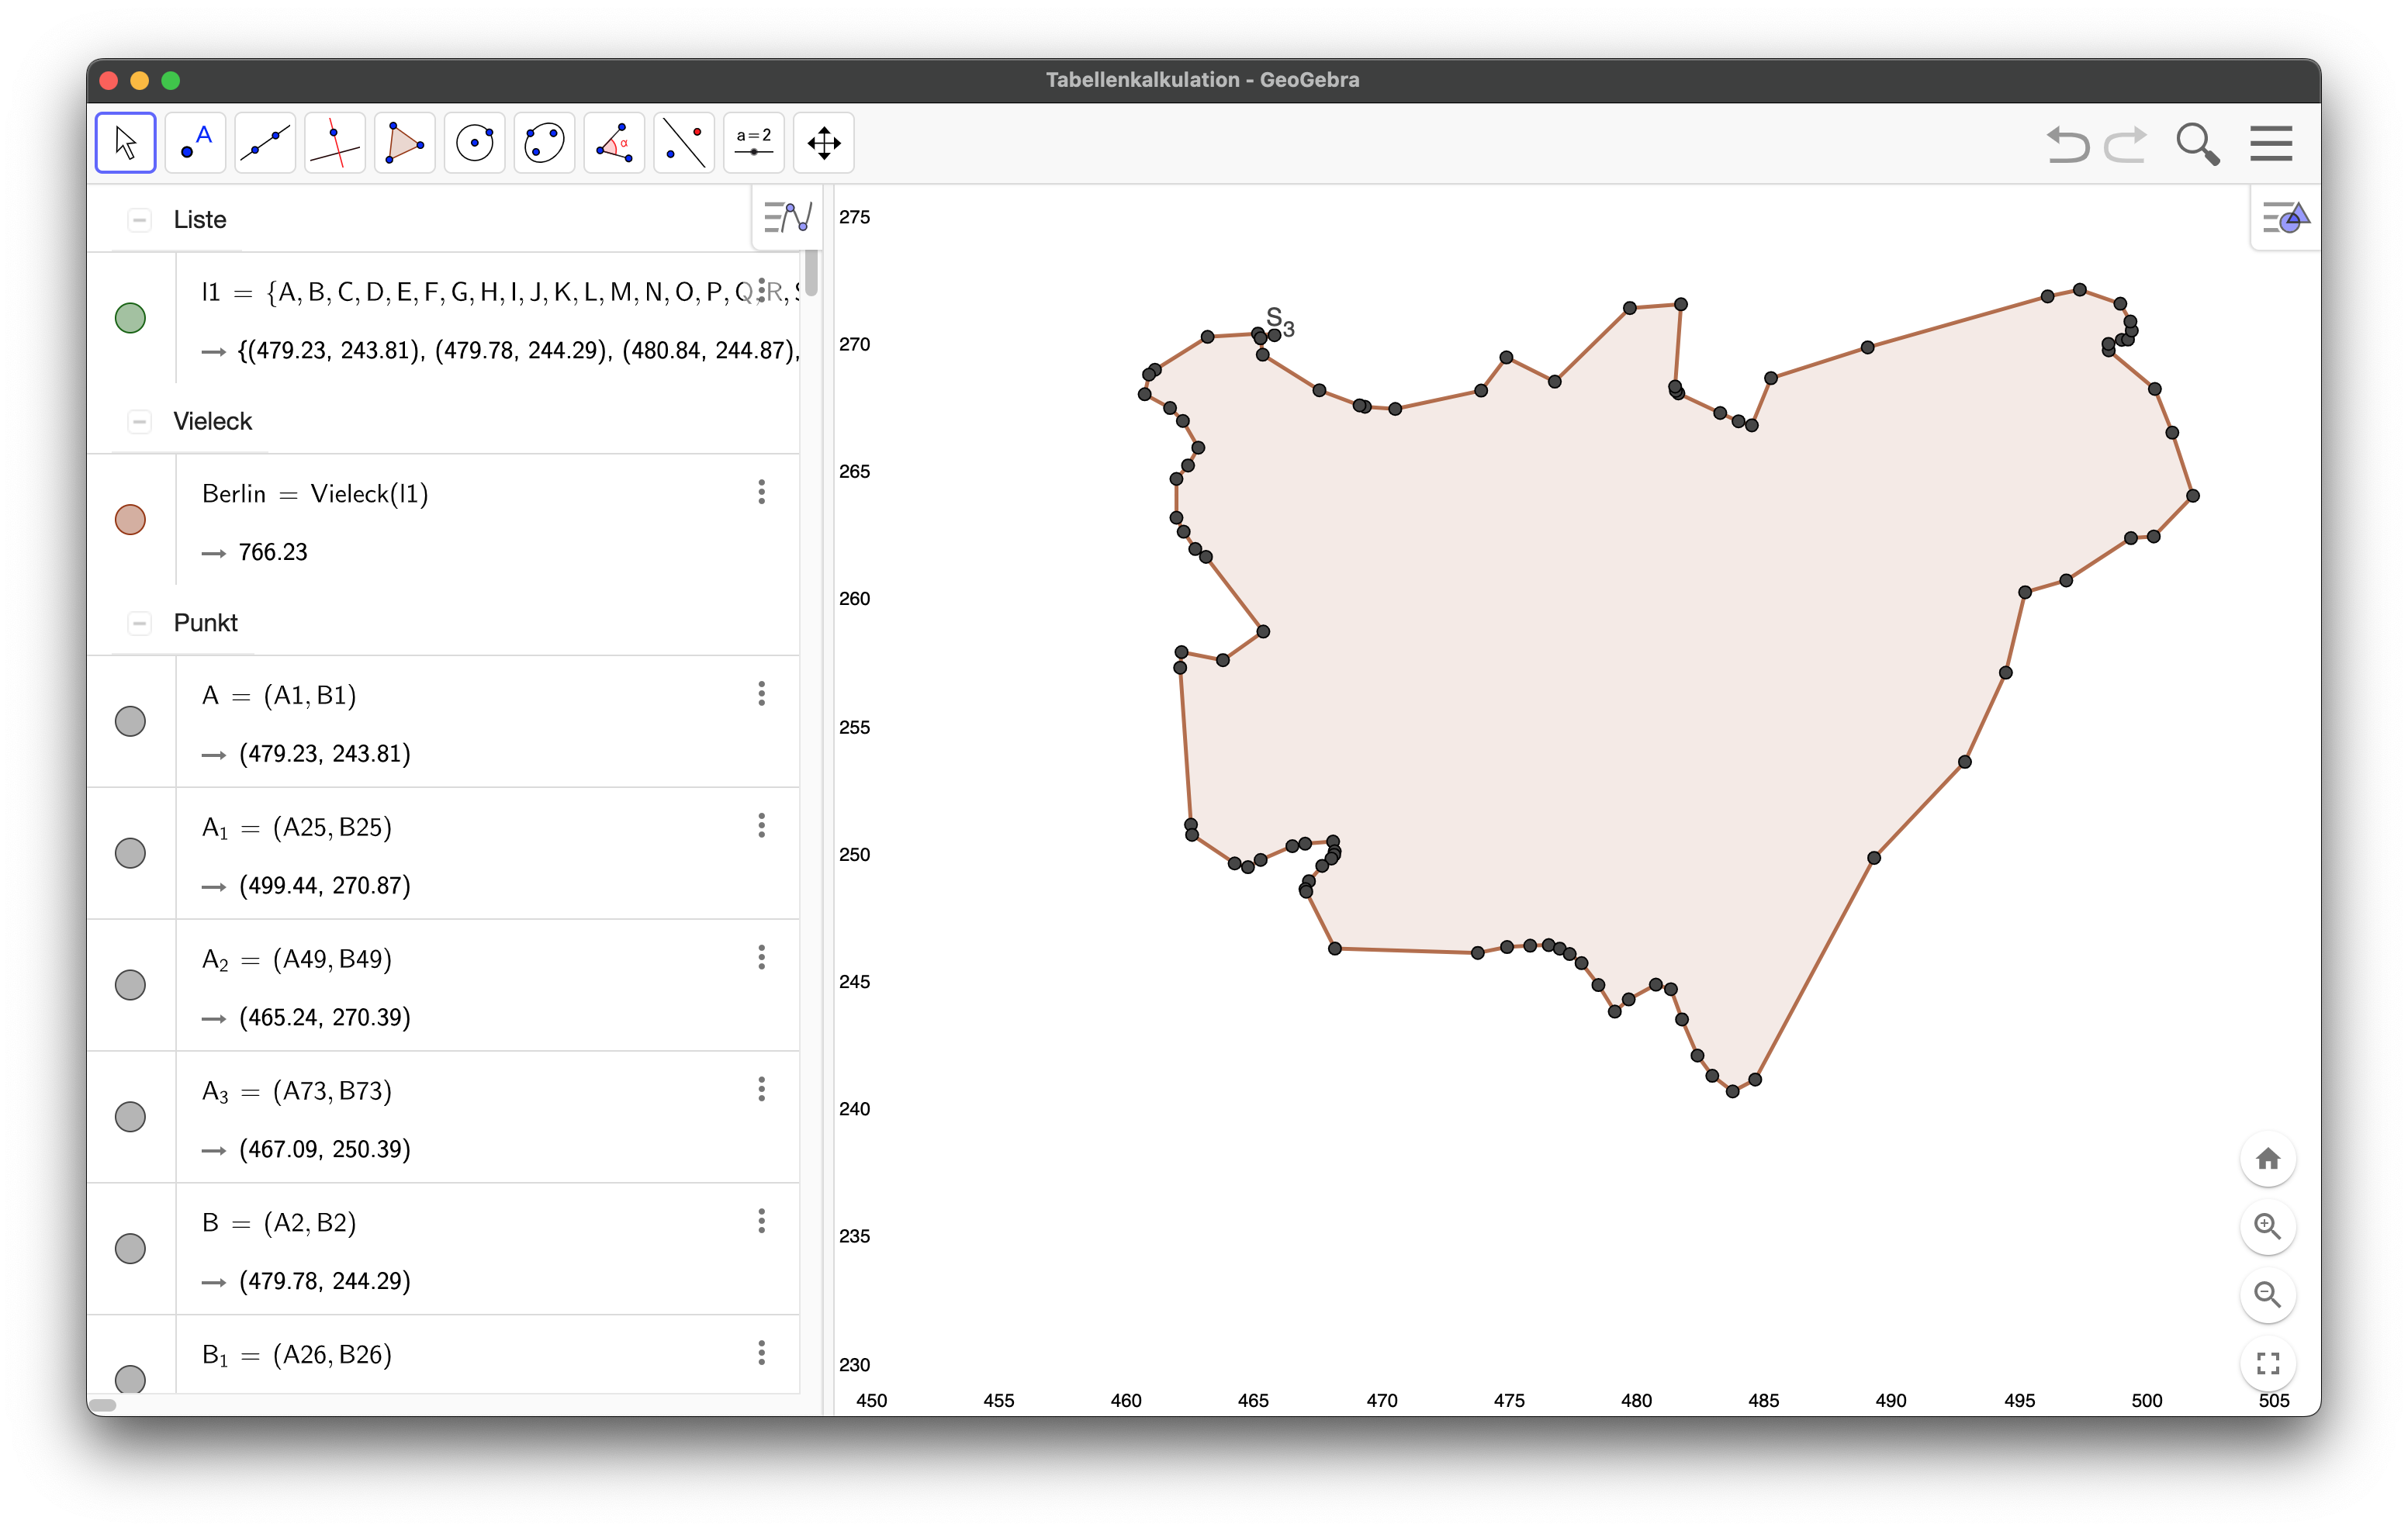
\includegraphics[scale=0.25]{GeoGebra Berlin.png}
    \caption{Berechnung der Fläche von Berlin mittels GeoGebra 6}
    \label{fig:geogebBerlin}
\end{figure}

Eine weitere Validierung wurde durch einen Abgleich mit anderen Pratikumsgruppen durchgeführt.
Hier kam der Hauptteil der befragten Gruppen auf das gleiche Ergebnis.

\end{document}
